% Bab II  Tinjauan Pustaka
\chapter{TINJAUAN PUSTAKA}

\section{Penelitian Terdahulu}
Minimal empat penelitian sejenis dalam kurun waktu tidak lebih dari 10 tahun terakhir. Cukup tuliskan nama peneliti, judul penelitian, dan kesimpulan hasilnya; satu paragraf untuk satu penelitian. Sumber boleh berasal dari skripsi, tesis, disertasi, maupun jurnal ilmiah.

\textit{Contoh kalimat bersitasi:} AlQahtani dan Alhassany (2013) membandingkan beberapa skema penjadwalan pada jaringan LTE. Penelitian tersebut sejalan dengan survei yang disusun oleh Capozzi et al. (2013). Kedua penelitian ini menjadi rujukan utama penelitian ini (AlQahtani \& Alhassany, 2013; Capozzi et al., 2013). Perbedaan dengan penelitian ini terletak pada …

Ringkasan penelitian terdahulu dapat disajikan dalam tabel perbandingan, seperti Tabel 2.1 (nama peneliti dan data pada tabel adalah contoh).

\begin{singlespace}
\begin{longtable}{|c|p{0.22\linewidth}|p{0.26\linewidth}|p{0.28\linewidth}|}
\caption{Contoh perbandingan penelitian terdahulu dengan penelitian ini}\\
\hline
\textbf{No.} & \textbf{Peneliti (tahun)} & \textbf{Metode/alat} & \textbf{Perbedaan dengan penelitian ini} \\
\hline
1 & Peneliti A (2022) & Sensor DHT11 dan Arduino Uno & Tanpa pengiriman data ke \textit{server} \\
\hline
2 & Peneliti B (2023) & Sensor DS18B20 dan ESP8266 & Hanya satu titik pengukuran \\
\hline
3 & Penelitian ini & Sensor DHT22 dan ESP32 & Tiga titik pengukuran dan dasbor \textit{web} \\
\hline
\end{longtable}
\end{singlespace}

\section{Landasan Teori}
Bagian ini hanya memuat teori yang mendukung penelitian. Sederhanakan uraian dari pustaka tanpa mengubah maksudnya, dan gunakan pustaka yang orisinal dan mutakhir.

\subsection{Teori Pertama}
Uraikan teori pertama beserta sitasinya, misalnya (Ghosh et al., 2010). Gambar dan tabel penjelas diberi nomor urut dan judul yang jelas. Gambar 2.1 adalah contoh gambar alat, yaitu sketsa papan mikrokontroler beserta keterangan bagian-bagiannya.

\textit{Contoh kalimat bersitasi:} Teori dasar sistem LTE dibahas secara menyeluruh oleh Ghosh et al. (2010). Rujukan pada halaman tertentu ditulis (Ghosh et al., 2010, hlm. 15). Kutipan langsung kurang dari 40 kata ditulis dalam tanda kutip dengan nomor halaman, misalnya menurut Andrews (2007, hlm. 3), “…kutipan langsung…”. Sumber yang dikutip dari sumber lain ditulis (Andrews, 2007, dalam Capozzi et al., 2013). Satu pernyataan yang didukung beberapa sumber dipisahkan dengan titik koma (Andrews, 2007; Xu \& Fischione, 2012).

\begin{figure}[H]
\centering
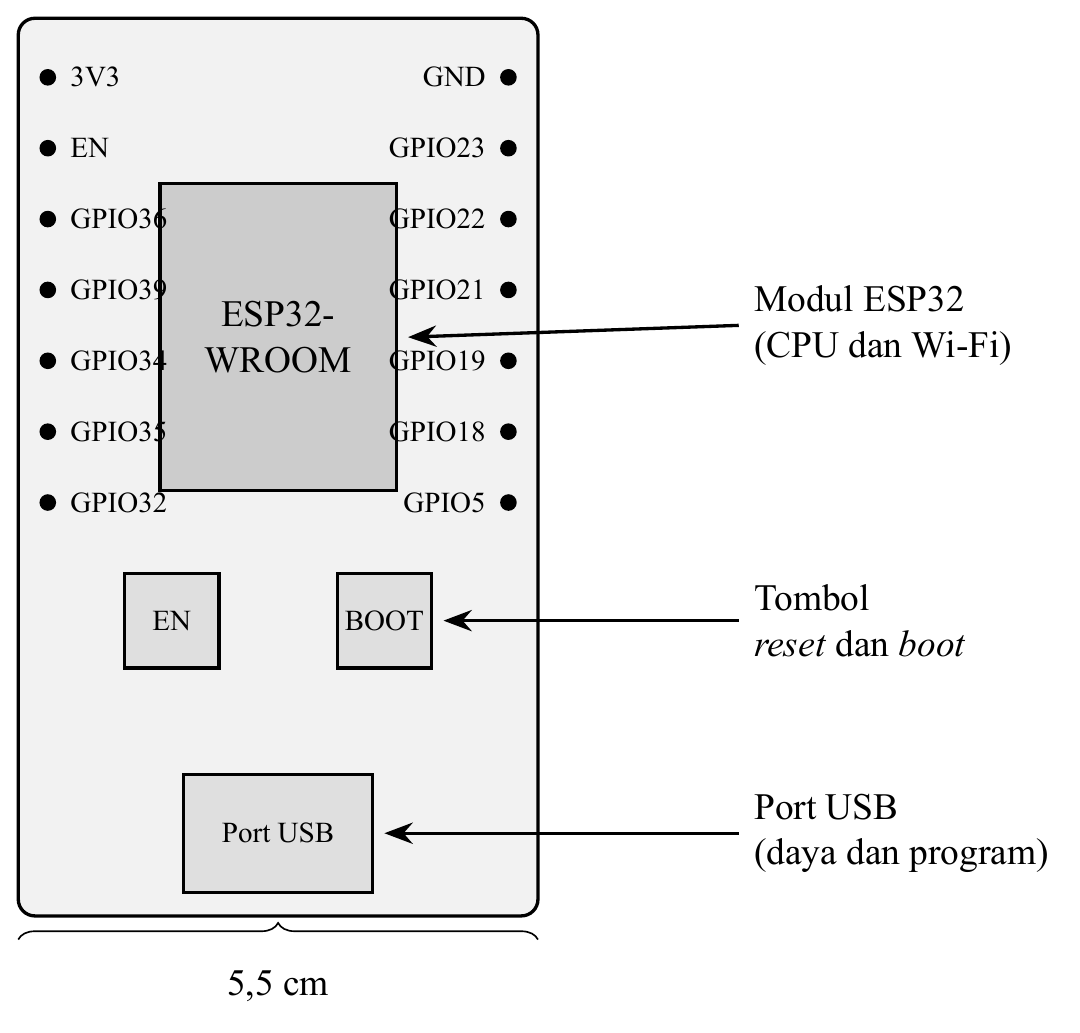
\includegraphics[width=0.55\textwidth]{../00-gambar/contoh-esp32.png}
\caption{Contoh sketsa papan mikrokontroler ESP32 beserta bagian-bagiannya}
\end{figure}

\subsection{Teori Kedua}
Uraikan teori kedua. Penulisan sitasi dua penulis: (Xu \& Fischione, 2012).

\textit{Contoh kalimat bersitasi:} Sumber buku terjemahan ditulis dengan nama penulis aslinya (Gaman \& Sherrington, 1994), artikel berbahasa Indonesia (Radiati, 2000), dan sumber tanpa penulis memakai judul (\textit{Panduan penulisan karya ilmiah}, 2020).

\section{Kerangka Pikir}
Kerangka pikir menggambarkan alur berpikir penelitian berdasarkan landasan teori dan penelitian terdahulu, dan dapat disajikan dalam bentuk diagram, seperti Gambar 2.2 (isi diagram adalah contoh).

\begin{figure}[H]
\centering
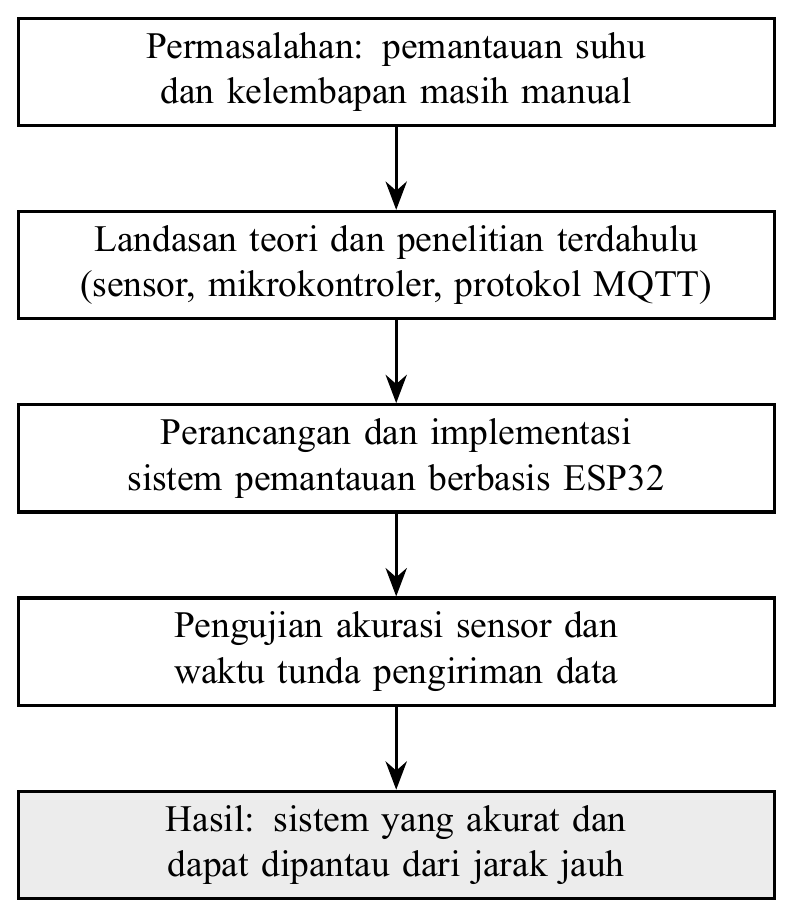
\includegraphics[width=0.5\textwidth]{../00-gambar/contoh-kerangka.png}
\caption{Contoh kerangka pikir penelitian}
\end{figure}
